\section{Runtime}\label{sec:runtime}
E6 measured a fixed 40-pair subset (seed 20261118; quotas 8/8/16/8 over the arms), 5 repetitions, sequential, one fresh process per job, on the Apple M4 Pro, \textbf{on battery power}. Both runs were flagged by the pre-registered load rule (run 1 load average 4.81 at start and 1.65 at the end; the repeat 1.44 and 2.24; transient spikes from other applications); 0 jobs failed; both runs are reported (Table~\ref{tab:e6}, Fig.~\ref{fig:e6}). V7-B's median per-pair wall time is 2.075~s against 1.310~s for B1: the median per-pair ratio is 1.595 (95\% CI $[1.584, 1.742]$) in wall time and 1.718 $[1.706, 1.844]$ in CPU time, and 1.018 $[1.014, 1.072]$ against B1+rep. V7-B therefore costs about $1.6\times$ B1, the interval excludes 1, and about as much as B1+rep. The median coefficient of variation across the five repetitions is 0.48\% (V7-B wall, run 1). Peak resident memory (tree maximum measured by the driver) has a median of about 26~MiB for V7-B and 28~MiB for B1, with a maximum of about 700~MiB for one pair; the engine does not log per-run memory. These figures are for one machine and a 40-pair subset and are not a scalability result.
\begin{table}[t]\centering\scriptsize\setlength{\tabcolsep}{3pt}
\caption{E6 runtime, 40-pair subset, 5 repetitions (V0 = default V7-B). Median per-pair wall time in seconds and median per-pair ratios with 95\% CI. Both runs were flagged by the pre-registered load rule; machine on battery power. Last column: 1-minute load average at start. Source: \path{results/v7b_phase2_summary/p2_e6_20261118_171723/timing/timing_summary.json} and \path{p2_e6b_20261118_174414/timing/timing_summary.json}.}\label{tab:e6}
\resizebox{\linewidth}{!}{%
\begin{tabular}{lrrrrrr}
\hline
Run & V0 wall & B1 wall & V0/B1 wall & V0/B1 CPU & V0/B1+rep wall & Load \\
\hline
run 1 & 2.075 & 1.310 & 1.595 [1.584, 1.742] & 1.718 [1.706, 1.844] & 1.018 [1.014, 1.072] & 4.81 \\
run 2 & 2.067 & 1.308 & 1.598 [1.586, 1.736] & 1.716 [1.706, 1.836] & 1.018 [1.015, 1.071] & 1.44 \\
\hline
\end{tabular}}
\end{table}

\begin{figure}[t]\centering
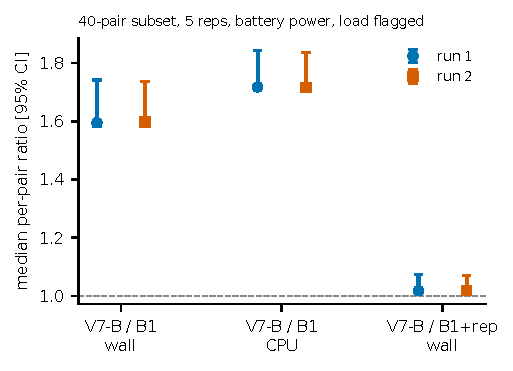
\includegraphics[width=0.92\columnwidth]{../../results/v7b_phase2_summary/figures/fig_p2_e6_overhead.pdf}
\caption{E6 median per-pair runtime ratios with 95\% CI for two runs; the dashed line is parity. Source: \path{results/v7b_phase2_summary/p2_e6_20261118_171723/timing/timing_summary.json} and \path{p2_e6b_20261118_174414/timing/timing_summary.json}.}\label{fig:e6}
\end{figure}
